\documentclass[tikz,border=2pt]{standalone}
\usepackage{amsmath,amssymb}
\usepackage{tikz}
\usetikzlibrary{arrows.meta}

\begin{document}
% A random interval [A, B] has random endpoints: each repetition of the experiment gives a
% different interval, and a fixed number theta may or may not be caught.
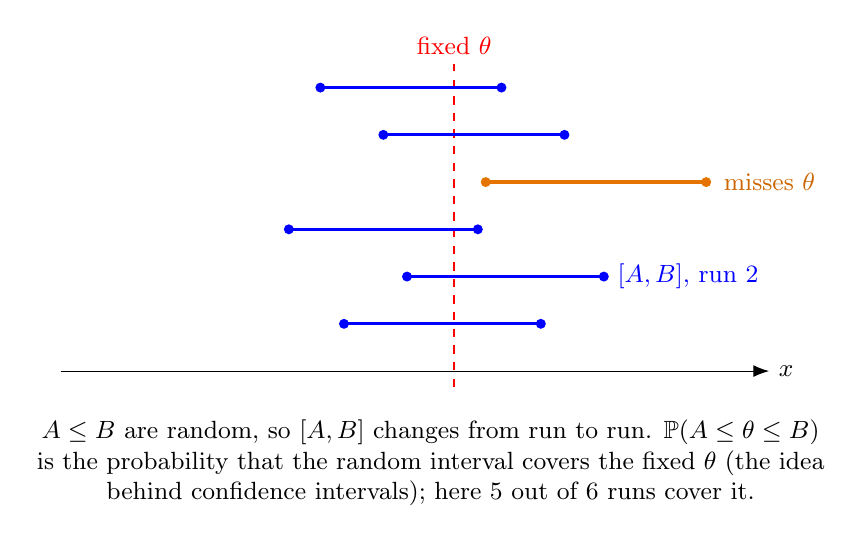
\begin{tikzpicture}[every node/.style={font=\small}, >={Latex[length=2mm]}]
	\draw[->] (0,0) -- (9.0,0) node[right] {$x$};
	\draw[red, dashed, thick] (5,-0.2) -- (5,3.9);
	\node[red, anchor=south] at (5,3.9) {fixed $\theta$};
	\foreach \a/\b/\y/\col in {3.6/6.1/0.6/blue, 4.4/6.9/1.2/blue, 2.9/5.3/1.8/blue, 5.4/8.2/2.4/orange!90!black, 4.1/6.4/3.0/blue, 3.3/5.6/3.6/blue} {
		\draw[\col, very thick] (\a,\y) -- (\b,\y);
		\fill[\col] (\a,\y) circle (1.8pt);
		\fill[\col] (\b,\y) circle (1.8pt);
	}
	\node[blue, anchor=west] at (6.95,1.2) {$[A,B]$, run $2$};
	\node[orange!80!black, anchor=west] at (8.3,2.4) {misses $\theta$};
	\node[anchor=north, align=flush center, text width=10cm] at (4.7,-0.5) {$A\le B$ are random, so $[A,B]$ changes from run to run. $\mathbb{P}(A\le\theta\le B)$ is the probability that the random interval covers the fixed $\theta$ (the idea behind confidence intervals); here $5$ out of $6$ runs cover it.};
\end{tikzpicture}
\end{document}
